\documentclass[letterpaper, 10pt, conference]{ieeeconf}
\IEEEoverridecommandlockouts
\overrideIEEEmargins
\usepackage[utf8]{inputenc}
\usepackage[T1]{fontenc}
\usepackage{amsmath,amssymb,graphicx,booktabs,float,gensymb,url}

\newcommand{\RNum}[1]{\uppercase\expandafter{\romannumeral #1\relax}}

\newcommand{\FitOne}{0.26748}
\newcommand{\FitTwoA}{0.26024}
\newcommand{\FitTwoB}{0.27534}
\newcommand{\DeltaBIC}{793.9}
\newcommand{\PeakTemp}{235.0}
\newcommand{\Prefactor}{1419.9}
\newcommand{\PeakCount}{1}
\newcommand{\FiveSelected}{138}
\newcommand{\FiveRecovered}{67}
\newcommand{\FiveTrials}{200}
\newcommand{\MatchedFalse}{0}
\newcommand{\BackgroundFalse}{200}
\newcommand{\BackgroundAlternative}{200}
\newcommand{\TransportFalse}{200}
\newcommand{\TransportAlternative}{171}
\newcommand{\StressTrials}{200}


\title{\LARGE \bf When Two Traps Look Like One:\\
A Computational Investigation of Defect-State Resolution}
\author{\textit{Aadi Bhattacharya}\\\textit{SNS F214 - Fundamentals of Solid State Physics}}

\begin{document}
\maketitle
\thispagestyle{empty}
\pagestyle{empty}

\begin{abstract}
Defects can trap mobile carriers and change how a semiconductor conducts when it is heated. This report asks whether two closely spaced trap levels can produce only one visible thermally stimulated conductivity peak. Using first order release kinetics, a Go program generates synthetic spectra motivated by measurements on $\beta$-In$_2$S$_3$ thin films. One and two trap fits are compared using the Bayesian Information Criterion. Two levels at $0.260$ and $0.275$ $eV$ produce one maximum, although both energies can be recovered in the baseline simulation. The results also show why fitting alone is not enough: an unmodelled background or temperature dependence can create a convincing but false second trap.
\end{abstract}

\section{INTRODUCTION}

We study the properties of a crystal while modelling a perfectly periodic crystal. Hence, the atomic arrangement and the periodic lattice potential determine the electronic properties of a crystalline semiconductor. However, an actual crystalline semiconductor is one with many structural imperfections, impurities, interfaces and vacancies, that can introduce additional electronic states in between band gaps.

These electronic states act as traps, holding an electron and temporarily removing them from mobile conduction states, bringing changes in carrier lifetimes, conductivity, photoconductivity responses, and recombination processes. This underlines the need of studying traps while studying the electrical performance of semiconductor materials.

$\beta$-In$_2$S$_3$, with it's defect spinel crystal structure has ordered cation vacancies. Experimentally prepared $\beta$-In$_2$S$_3$ thin films may also contain additional electrically active defects. {Pai \emph{et al.}} \cite{pai} investigated the defect related electronic states in spray pyrolysed $\beta$-In$_2$S$_3$, using thermally stimulated conductivity measurements. Multiple activation energies were reported with different proposed  defects.

In thermally stimulated current spectroscopy measurements, a semiconductor (excited in prior,) is heated while it's electrical conductivity is monitored. Thermal emissions from occupied localised electronic states can produce characteristic peaks in the measured responses. The specific temperatures and shapes of these peaks contain valuable information about the trapping process.

When two defect levels have similar thermal release characteristics, an issue arises. They might overlap sufficiently to produce a single maximum, despite there being two active electronic trapping populations.

This investigation delves into three related questions: Are two traps sufficient to produce a single apparent TSC peak? Can their individual activation energies still be recovered computationally? Is a successful mathematical fit be sufficient in establishing the existence of distinct physical defects?

\section{SEMICONDUCTOR PHYSICS}
\subsection{Crystal Structure and Bonding}

Indium Sulfide, In$_2$S$_3$ is a \RNum{3}-\RNum{6} compound semiconductor that exists as several structural polymorphs, with the $\beta$ phase having a tetragonal defect spinel structure. It has the crystallographic space group $I4_1/amd$. \cite{pistor}

A tetragonal bravais lattice has two equal lattice parameters, $a=b$, and a third generally unequal parameter $c$. The axes are mutually perpendicular. For the $\beta$-In$_2$S$_3$ structure investigated by {Pistor \emph{et al.}} \cite{pistor}, we approximately get parameters $a = b = 7.623 \text{\AA}$, and $c = 32.358 \text{\AA}$.

We have a crystal structure having a Sulfur framework with Indium ions occupying tetrahedrally and octahedrally co-ordinated sites. For the unoccupied cation positions, their ordering is associated with that of a tetragonal structure.

$\beta$-In$_2$S$_3$ involves both ionic and covalent bonding characteristics, which arises from the interactions between Indium and Sulfur electronic states. These interactions, along with the periodicity and symmetry of the lattice, determine the electronic band structure.

These crystallographically vacant sites aren't inherently the same as electrically active traps, with no guarantee for a localised electronic level with a particular thermal activation energy. Such electronic consequences depend on the local environment, charged states and structural relaxations.

\subsection{Bands, Effective Mass and Carrier Statistics}
According to Bloch's theorem, an electronic wavefunction in a periodic potential can be written as:
$$ \psi_{n,k}(r)=u_{n,k}(r)\exp{(i k \cdot r)}. $$
Where $u_{n,k}(r)$ has the periodicity of the crystal lattice and $k$ is the electron wavevector.

Solving for $u_{n,k}$ produces the energy eigen values $E_n(k)$ which gives us the allowed electronic bands.

At temperature being equal to $0K$, the highest occupied electronic band is conventionally taken to be the valence band, with the next available band being the conduction band. The fundamental band gap is defined as the minimum energy required to excite an electron from the valence maximum to the conduction band minimum.

For a direct band gap semiconductor, these band extremas occur at the same crystal wavevector. In an indirect band gap semiconductor, they occur at different crystal wavevectors, requiring momentum conservation via phonon participation in an optical transition.

Theoretical calculations of $\beta$-In$_2$S$_3$ have identified it to have an indirect fundamental band gap. \cite{zhao}. Experimental optical measurements yield different band gap values and different transitions.

{Pai \emph{et al.}}\cite{pai} reported an optical absorption gap of approximately $2.6 eV$ for their spray pyrolysed $\beta$-In$_2$S$_3$ films. This reported value should not be equated with the fundamental gap of an ideal crystal calculated using electronic structure methods.

The response of a carrier to an externally applied force depends on the curvature of the corresponding energy band. The group velocity is given by:

$$ v_g = \frac{1}{\hbar} \frac{dE}{dk}$$

With the force being given as:

$$ \hbar \frac{dk}{dt} = F $$

Differentiating and comparing the result with Newton's Second Law gives:
$$ \frac{1}{m^*}=\frac{1}{\hbar^2}\frac{d^2 E}{dk^2} $$

Here $m^*$ is the effective mass in a one dimensional band approximation. In an anisotropic crystal, the effective mass is usually described by a second-rank tensor.

A strongly curved energy band corresponds to a smaller effective mass in the corresponding direction, while a softer band corresponds to a larger effective mass.

Effective mass influences acceleration and contributes to the density of available electronic states. It does not independently determine carrier mobility, which also depends on scattering mechanisms.


Occupation of electronic states at thermal equilibrium follows Fermi-Dirac statistics, where the probability that an electronic state is occupied at agiven temperature $T$ is given as:

$$ f(E)=\frac{1}{1+\exp[(E-E_F)/(k_BT)]} $$

For non-degenerate semiconductors we approximate carrier concentrations with:

$$ n = N_C \exp{[-(E_C-E_F)/(k_BT)]} $$
$$ p = N_V \exp{[-(E_F-E_V)/(k_BT)]} $$

Where $N_C$ and $N_V$ are the effective densities of states for the conduction and valence bands, and $E_C$ and $E_V$ are the energy for the conduction and valence bands.

\subsection{Charge Carriers and Transport}

Electrical transport in semiconductors is primarily described through drift and diffusion currents.

Drift occurs when an electric field exerts a force on mobile charge carriers. In the low field regime, the carrier drift velocity is proportional to the applied electric field, with mobility being the proportionality coefficient.

$$ \sigma=q(n\mu_n+p\mu_p) $$

Where $q$ is the elementary charge, $n$ and $p$ are mobile carrier concentrations, and $\mu_n$ and $\mu_p$ are their corresponding mobilities.

Diffusion occurs with spatial variations in carrier concentration. Diffusion tends to redistribute carriers from regions of higher concentrations to lower ones, it's contribution depends on the carrier density gradient.

$$ J_n=qn\mu_n\mathcal{E}+qD_n\nabla n $$
$$ J_p=qp\mu_p\mathcal{E}-qD_p\nabla p $$

The difference in the signum of the later term comes from difference in polarity in the charges of the holes and electrons.

For non degenerate carriers in an appropriate near equilibrium regime, mobility and diffusion coefficients are related through the Einstein's relation:

$$ \frac{D}{\mu} = k_B\frac{T}{q} $$

Defect states influence transportation because trapping changes the population of mobile carriers available for conduction.

An electron excited into the conduction band can be captured by a localised state. Whence trapped, it no longer can participate in ordinary band conduction. Subsequent thermal emission can return it to the conduction band, where it might drift, diffuse, become trapped again, or recombine.

Hence, measured electrical current during thermal stimulation depends on mobility, recombination lifetime, electric field, sample geometry, the rate of carrier release from traps and additional trapping processes.

\section{DEFECTS AND THERMALLY STIMULATED CONDUCTIVITY}
Pai \emph{et al.} used spray pyrolysed $\beta$-In$_2$S$_3$, varying the Indium/Sulfur concentration ratio in the depostion ratio. \cite{pai}.

The films were deposited at a substrate temperature approximately equal to $300 \degree C$ with thicknesses in the order of $1 \mu m$. Their reported optical gap was approximately equal to $2.6 eV$, and hot probe measurements indicated n type conductivity.

For Thermally stimulated current spectroscopy measurements, the samples were cooled down to $100K$ in a vacuum of $10^-2 Torr$. Thereafter, they were illuminated with white light at a power density of $10 mW/cm^2$ for $60$ seconds, to create a photoexcited carrier population.

Following this illumination, the temperature was increased at a constant rate of $3 K/min$. Electric current was recorded during the heating process under a bias of $30 V$ with an electrode separation of $0.5 cm$.

The authors reported the following datum.

\begin{table}[H]
\caption{Reported thermal activation energies in $\beta$-In$_2$S$_3$ \cite{pai}.}
\label{tab:traps}
\centering\footnotesize
\begin{tabular}{@{}ccc@{}}\toprule
Activation Energy & Peak Temperature & Proposed origin\\\midrule
0.10 eV & 160 K & In vacancy\\
0.26 eV & 230 K & Cl impurity\\
0.43 eV & 320 K & S vacancy\\
0.82 eV & 450 K & O substitution on a S site\\\bottomrule
\end{tabular}
\end{table}

The $0.10 eV$ feature became more prominent in Indium poor preparations, while the $0.43 eV$ contribution generally weakened with increasing Sulfur concentration.

The authors also employed Gaussian fitting to separate overlapping components of the TSC response. While such fitting can help distinguish contributions with different temperature dependence, identifying a fitted component with a unique microscopic defect requires additional physical justification.

\subsection{First-Order Thermal Release Model}
A trapped electron must get enough energy to escape from a localised state into an available mobile state.
In a simplified thermally activated model the probability of escape per unit time is described by the Arrhenius equation:

$$ e(T)=s\exp\!\left(-\frac{E_a}{k_BT}\right) $$

Where $E_a$ is the activation energy and $s$ is the effective emission prefactor.

Let $n_t(t)$ represent the concentration of occupied traps. If retrapping is neglected and each trapped electron escapes independently, the trap population satisfies the following first order differential equation:

$$ dn_t/dt = -e(T)n_t $$

Where the negative signum indicates that thermal emission reduces the number of occupied states.

For a constant heating rate given by $\beta = dT/dt$, the chain rule gives $\frac{dn_t}{dT} = -\frac{e(T)}{\beta}n_t$. Thereafter, separating variables and integrating from an intial temperature of $T_0$,

$$ n_t(T) = n_{t_0} exp{[-\frac{1}{\beta} \int_{T_0}^T e(\theta)d\theta]} $$

The instantaneous rate of carrier release is the product of the thermal emission probability and the remaining trapped population,

$$ F(T) = e(T)n_t(T) $$

At low temperatures, the emission rate is strongly suppressed. As heating proceeds, carrier emission increases, causing the release flux to increase.

Eventually, the trapped population becomes depleted. The reduction in occupied states outweighs the increasing thermal emission probability, causing the release flux to decrease.

The competition between these processes produces a maximum in the thermal release curve.

To find the temperature of maximum release, we set the logarithmic derivative of $F(T)$ to zero:

$$ \frac{d ln F}{dT} = \frac{E_a}{k_B T^2} - \frac{e(T)}{\beta} = 0 $$

At the peak temperature $T_m$,

$$ e(T_m) = \beta \frac{E_a}{k_B T_m^2} $$

Substituting the Arrhenius emission expression gives

$$ s \exp[-E_a/(k_B T_m)] = \beta \frac{E_a}{k_B T_m^2} $$

This relationship connects the peak temperature to the activation energy, heating rate, and emission prefactor under ideal first order assumptions.

For two independent trap populations, the release fluxes can be added:

$$ F_{total}(T) = e_1(T)n_{t_1}(T) + e_2(T)n_{t_2}(T) $$

When carrier collection is sufficiently quick and the effective mobility and collection factors are constant, the excess TSC signal may be approximated as proportional to this combined release flux.

\subsection{Limitations of the First-Order Approximation}

The usefulness of the first order approach lies in providing a convenient way to establish the relationship between the thermal activation energy and temperature dependent release signal.

Yet, the measured current does not usually correspond to the rate of the instantaneous carrier release.

In their general analysis of the thermally stimulated conductivity Dussel and Bube \cite{dussel} took into account the competition between the thermal emission, retrapping, recombination, and variation of the carrier lifetime.

The released carrier may be trapped again by some other empty state before its recombination or transport; Retrapping slows down the process of carrier release and affects the temperature behavior of the free carrier concentration. In addition, the carrier lifetime could vary during the heating due to changing occupation of the trapping and recombination sites.

These mechanisms result in broadening, shifting of TSC peak maxima, and alteration of the activation energies of peaks by the simple peak analysis procedures.

Therefore, the model based on the first order carrier release should be regarded as a convenient approximation rather than a microscopic model of electrical transport.

\section{COMPUTATIONAL METHOD}

The computational investigation was implemented in Go to generate synthetic TSC signals and evaluate the ability of numerical fitting procedures to distinguish closely spaced trap levels.

The complete Go implementation, numerical experiments, and reproducibility instructions are publicly available at \url{https://github.com/aadi-bhattacharya/trap-electronics}.

The forward model uses the first order release equations to calculate the temperature dependent contribution of each trap population.

A uniform temperature grid extending from $100 K$ to $340 K$ with increments of $0.5 K$ was employed. The heating rate was fixed at $0.05 K/s$, matching the rate used by Pai \emph{et al.}\cite{pai}

The baseline experiment used two activation energies:

$$ E_1 = 0.260 eV $$
$$ E_2 = 0.275 eV $$

The first value corresponds to a reported activation energy in $\beta-In_2S_3$, while the second is a hypothetical level introduced specifically to examine peak overlap.

A common effective emission prefactor of approximately $1.42 \times 10^3 s^-1$ was calibrated from the first order peak equation so that the $0.260 eV$ trap generated a maximum near $230 K$.

The combined release signal was normalized and synthetic Gaussian noise was added with a standard deviation equal to $1\%$ of the normalised peak amplitude.

Two mathematically competing models were then fitted to the generated data, one with one thermally active trap and another with two independent traps.

The fit quality was evaluated using the residual sum of squares:
$$ \text{RSS} = \sum_{j} \left[ y_{\text{observed}}(T_j) - y_{\text{model}}(T_j) \right]^2 $$


To account for the greater complexity of the two trap model, the Bayesian Information Criterion was calculated as:

$$ \text{BIC} = N \ln(\text{RSS}/N) + k \ln N $$

Where $N$ is the number of sampled observations and $k$ is the number of fitted model parameters.

The preferred model was determined by comparing the difference:

$$ \Delta \text{BIC} = \text{BIC}_{one-trap} - \text{BIC}_{two-trap} $$

A positive difference favors the two trap hypothesis. This investigation used a threshold of $\Delta\mathrm{BIC}$ greater than $10$ to indicate a strong model preference.

Repeated simulations were also performed at different energy separations. Accurate recovery was evaluated using a specified tolerance of $2 meV$ for the fitted activation energies.

\section{RESULTS AND RESEARCH CHALLENGE}
\begin{figure}[H]
\centering
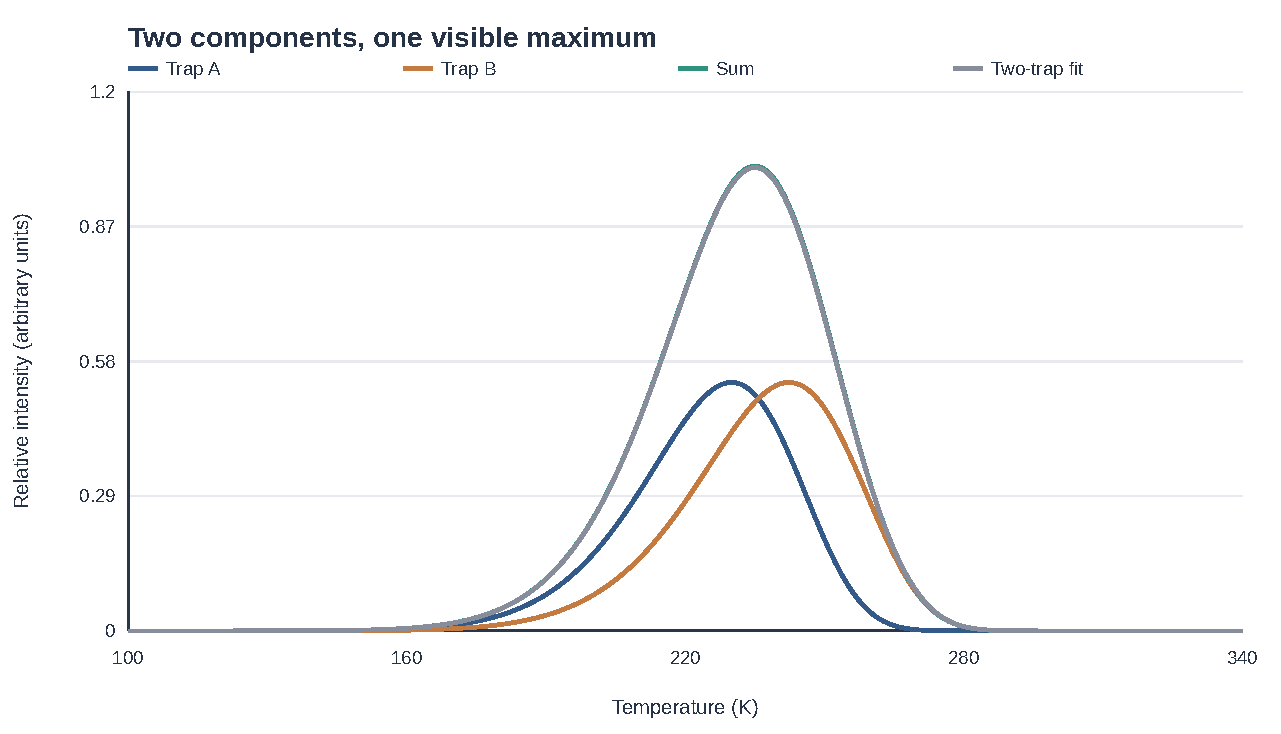
\includegraphics[width=.98\columnwidth,height=1.55in,keepaspectratio]{figures/demo.pdf}
\caption{Synthetic Go-generated components and total on a common scale. One visible maximum does not imply one generating trap.}
\label{fig:demo}
\end{figure}


\subsection{A Single Peak from Two Traps}
Figure~\ref{fig:demo} shows the two simulated contributions and their sum. The activation energies differ by $15 meV$, but the combined curve has only one maximum, at $\PeakTemp\,\mathrm{K}$. A one-trap fit gives $\FitOne\,\mathrm{eV}$, between the two input energies. The two-trap fit recovers $\FitTwoA$ and $\FitTwoB\,\mathrm{eV}$, close to the chosen values. The difference in BIC is approximately $\DeltaBIC$, in favour of the two-trap model.

Thus, one visible maximum is not enough to conclude that only one trap is present. This successful recovery also has a clear qualification: the data and fitted models use the same first-order physics, and the effective emission prefactor is held fixed.

\subsection{How Much Separation Is Enough?}
To test whether the result survives noise, the Go program repeats the fit for $200$ synthetic datasets at each energy separation. The two-trap model is selected when $\Delta\mathrm{BIC}>10$; recovery is counted only when both energies are also within $2 meV$ of their inputs. Table~\ref{tab:resolution} gives the counts. At $5 meV$, two traps are preferred in $\FiveSelected$ of $\FiveTrials$ trials, but the energies are both recovered in only $\FiveRecovered$. At $10 meV$, the corresponding counts are $200$ and $199$. Detecting that the curve needs more than one component is therefore not the same as measuring both activation energies reliably.

\begin{table}[H]
\caption{Go-generated results, 200 synthetic noise trials per condition.}
\label{tab:resolution}
\centering\footnotesize
\begin{tabular}{@{}ccc@{}}\toprule
Separation (meV) & Two traps preferred & Both recovered\\\midrule
2 & 0/200 & 0/200\\
5 & 138/200 & 67/200\\
10 & 200/200 & 199/200\\
15 & 200/200 & 200/200\\
20 & 200/200 & 200/200\\\bottomrule
\end{tabular}
\end{table}

\subsection{A Good Fit Can Still Be Wrong}
A final check starts with just one simulated trap. When the generating and fitting models agree, the program incorrectly selects two traps in none of the 200 trials. The result changes when the fit ignores a small constant background or a temperature dependent weighting of the signal: a restricted two trap fit is then preferred in 200 out of 200 trials in each case. A one trap model that includes the missing background is preferred over the two-trap alternative in all 200 background trials; allowing for temperature weighting does so in 171 trials. The weighting is an illustrative model assumption, not a measured mobility law for $\beta$-In$_2$S$_3$.

These tests bring out the main research challenge. An extra fitted component may be describing a second trap, but it may also be compensating for physics left out of the model. The reported resolution depends on noise, the chosen kinetic equations and which parameters are allowed to vary. It should not be taken as a universal experimental limit or as proof of particular microscopic defects.

\section{FUTURE PROSPECTS AND CONCLUSION}
\subsection{Future Prospects}
Better identification of trap levels could help researchers distinguish useful carrier transport from trapping and recombination losses in thin film devices. This is relevant to $\beta$-In$_2$S$_3$ photodetectors and solar cell structures, where defects can affect the electrical response. Recent work on sulfur vacancies in $\beta$-In$_2$S$_3$ photoelectrodes also shows why controlling defect populations matters \cite{kaur}. A useful next experiment would compare spectra measured at several heating rates, with similar initial trap filling. On the computational side, the Go model could be extended to fit the emission prefactor and include retrapping and temperature dependent mobility rather than treating them as fixed or negligible.

\subsection{Conclusion}
The calculations show that two trap populations can give a single maximum in a TSC spectrum. That does not necessarily mean the levels are unresolvable: in the baseline synthetic example, the two trap fit recovers both input energies. The repeated trials show that choosing a two trap model is easier than determining both energies accurately. More importantly, the stress tests show that missing background or transport physics can make a single trap look like two. The method is therefore useful for testing resolution, but it cannot by itself establish the number or chemical identity of defects in a real sample.

\begin{thebibliography}{5}
\bibitem{pai} R. R. Pai \emph{et al.}, ``Defect characterization of spray pyrolised $\beta$-In$_2$S$_3$ thin film using thermally stimulated current measurements,'' \emph{J. Mater. Sci.}, vol. 40, pp. 741--746, 2005, doi: 10.1007/s10853-005-6315-8.
\bibitem{pistor} P. Pistor \emph{et al.}, ``Structure reinvestigation of $\alpha$-, $\beta$- and $\gamma$-In$_2$S$_3$,'' \emph{Acta Crystallogr. B}, vol. 72, pp. 410--415, 2016, doi: 10.1107/S2052520616007058.
\bibitem{zhao} Z. Zhao \emph{et al.}, ``Band-edge electronic structure of $\beta$-In$_2$S$_3$: The role of s or p orbitals of atoms at different lattice positions,'' \emph{ChemPhysChem}, vol. 13, pp. 1551--1556, 2012, doi: 10.1002/cphc.201100968.
\bibitem{dussel} G. A. Dussel and R. H. Bube, ``Theory of thermally stimulated conductivity in a previously photoexcited crystal,'' \emph{Phys. Rev.}, vol. 155, pp. 764--779, 1967, doi: 10.1103/PhysRev.155.764.
\bibitem{kaur} N. Kaur, ``Sulfur vacancy-driven charge carrier dynamics in $\beta$-In$_2$S$_3$ photoelectrodes,'' \emph{J. Alloys Compd. Commun.}, vol. 11, art. 100214, 2026, doi: 10.1016/j.jacomc.2026.100214.
\end{thebibliography}
\end{document}
